\documentclass[tikz, border=3mm]{standalone}
\usepackage{tikz}
\usetikzlibrary{arrows.meta, positioning, decorations.markings}

\begin{document}
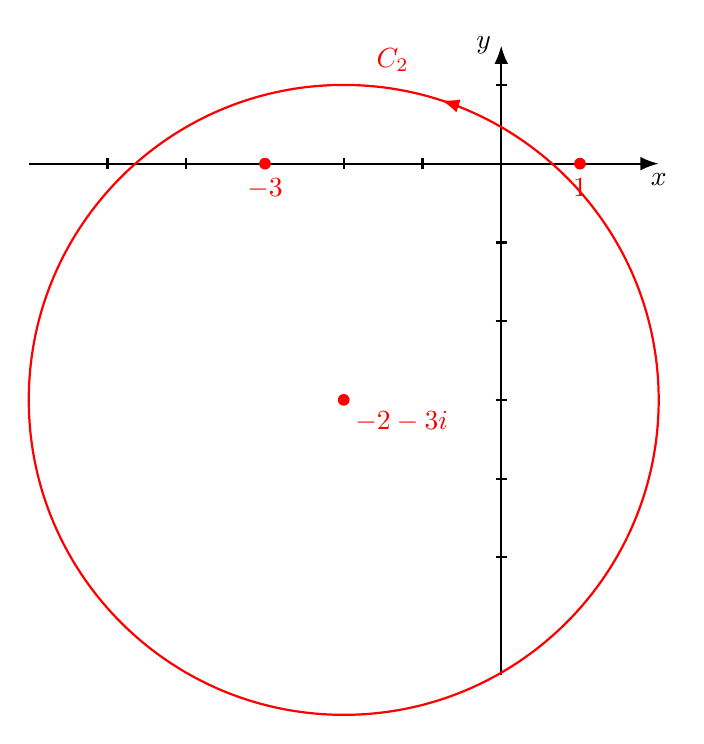
\begin{tikzpicture}[
    >=Latex, % Set default arrow tip style
    axis/.style={->, thick}, % Style for axes
    pathstyle/.style={red, thick}, % Style for the ellipse path
    labelstyle/.style={red}, % Style for labels
    tick/.style={thick}, % Style for tick marks
    dot/.style={fill=red, circle, inner sep=1.5pt}, % Style for red points
midarrowL/.style={
        decoration={markings, mark=at position 0.2 with {\arrowreversed{Latex}}},
        postaction={decorate}
    },
    midarrow/.style={
        decoration={markings, mark=at position 0.2 with {\arrow{Latex}}},
        postaction={decorate}
    }	
]

    % Define ellipse parameters (approximated from image)
    % Center seems slightly left of origin, maybe (-1, 0)
    % x-radius seems to be 2 (from -3 to 1)
    % y-radius seems to be 3 (judging by height)
    \coordinate (Center) at (-1, 0);
    \def\xrad{2}
    \def\yrad{3}

\def\radius{4}
    % Axes (adjust limits)
    \draw[axis] (-6, 0) -- (2, 0) node[below] {$x$};
    \draw[axis] (0, -6.5) -- (0, 1.5) node[left] {$y$};

    % Draw the red ellipse with counter-clockwise arrow
   % \draw[pathstyle,
   %     postaction={decorate, decoration={markings,
   %         % Arrow near top-left (pos=0.6 approx)
   %         mark=at position 0.6 with {\arrow[red, thick]{<}}
   %     }}
   % ] (Center) circle [x radius=\xrad, y radius=\yrad];

\draw[pathstyle, midarrow, red] (-2,-3) circle (\radius); % Arrow at pos 0.375 (top-left)
    % Ticks on axes
    \foreach \x in {-3, -2, -1, 1, -3, -4, -5} {
        \draw[tick] (\x, -2pt) -- (\x, 2pt);
    }
    \foreach \y in {-3, -2, -1, 1, -4, -5} {
        \draw[tick] (-2pt, \y) -- (2pt, \y);
    }

    % Points marked on the axes/curve
    \node[dot] at (-3, 0) {};
    \node[dot] at (1, 0) {};
    %\node[dot] at (-1, \yrad) {};  % Approx top point on ellipse
    %\node[dot] at (-1, -\yrad) {}; % Approx bottom point on ellipse
    \node[dot] at (-2, -3) {}; % Point for 2-3i label

    % Labels
    \node[labelstyle, below=2pt] at (-3, 0) {$-3$};
    \node[labelstyle, below=2pt] at (1, 0) {$1$};
    \node[labelstyle, below right=1pt] at (-2,-3) {$-2-3i$}; % Label text as shown
    \node[labelstyle, above left=2pt] at (-1, 1) {$C_2$}; % Label curve near arrow

\end{tikzpicture}
\end{document}